\documentclass[../tesi.tex]{subfiles}
\begin{document}
\chapter{Introduzione}

Il Machine Learning sta diventanto molto diffuso nelle realtá aziendali IT e non solo, essenziale per fare previsioni basati su calcoli statistici.\\
In questo testo andremo ad analizzare due casi di studio per comprendere le modalitá in cui l’appredimento automatico  interagisce in diversi ambiti, al fine di illustrare una serie di strumenti che permettono di orchestrare in maniera automatica i flussi di lavoro del Machine Learning.\\
Metteremo in relazione i casi di studio analizzati con altri due compagni di corso, con l’obiettivo di individuare un'invariante il piú possibile automatizzata che possa permettere di sfruttarne i benefici.\\
Questa analisi viene eseguita confrontando i diversi passaggi ``fondamentali'' tra i casi di studio presi in considerazione. \\
Una volta analizzate le differenze e le analogie presenti nei diversi casi di studio, tracceremo una linea di ``workflow generica'', evidenziando le fasi di processo comuni, i quali diventeranno essenziali per capire come cercare di automatizzare la gestione dei flussi di lavoro del Machine Learning.\\
Senza la pretesa di essere completi studieremo e confronteremo un insieme di \Gls{framework}, che permettono di orchestrare in maniera automatica diversi flussi di lavoro che, come vedremo, saranno simili al "workflow generico'' illustrato in fase di analisi.\\
Per illustrare e capire il funzionamento di diversi strumenti di orchestrazione è necessario, in prima istanza, analizzare e confrontare come i processi di ML agiscono nei diversi casi di studio utilizzando in tal modo un approccio bottom-up.

\newpage
\section{Intelligenza Artificiale}
\chapquote{``We spend a great deal of time studying history, which, let’s face it, is mostly the history of stupidity. So it’s a welcome change that people are studying instead the future of intelligence. "}{Stephen Hawking}{}
L’intelligenza è l’abilitá di imparare dalle esperienze, per applicare le conoscenze volte a risolvere dei problemi, adattandoli in differenti ambiti.\\
L’intelligenza artificiale è un ramo dell’informatica che si occupa di studiare metodologie e tecniche in grado di sviluppare programmi software capaci di fornire all’elaboratore elettronico prestazioni che possono apparire di pertinenza esclusiva dell’intelligenza umana.\\
Possiamo osservare diverse tipologie di AI:
\begin{itemize}
  \item Thinking Humanly
  \item Action Humanly
  \item Thinking Rationally
  \item Action Rationally
\end{itemize}
La differenza in questi 4 campi mette in relazione il pensare dell’umano al risultato(``\textit{action}") oppure al processo(``\textit{thinking}") del sistema intelligente.\\
Nei primi due casi il sistema intelligente viene paragonato alla capacità di risolvere un problema o di svolgere un’azione in maniera simile a quella di un umano.\\
Mentre gli ultimi due campi svolgono un’azione seguendo un processo razionale.

\section{Apprendimento Automatico}
L’apprendimento automatico(\textit{Machine Learning,ML}) è un ramo dell’intelligenza artificiale, che raccoglie metodi in grado di migliorare la performance di un algoritmo, autonomamente, nell’identificare pattern di dati.\cite{enwiki:1046345973}\\
L’apprendimento automatico cerca di costruire algoritmi e modelli che possono imparare a prendere decisioni senza dati con regole predefinite. Gli algoritmi di ML esistenti si suddividono in tre categorie:
\begin{itemize}
  \item \textbf{Supervised Learning}: algoritmi che cercano di condurre una classificazione o regressione su dati targettizzati.
  \item \textbf{Unsupervised Learning}, si focalizzano sulla classificazione di semplici insiemi in gruppi 
  \item \textbf{Reinforcement Learning}, gli agenti imparano la migliore azione da eseguire che ti portino al beneficio superiore
\end{itemize}
L'\textit{Apprendimento supervisionato} mira a istruire il sistema in modo da permettergli di elaborare automaticamente previsioni sui valori di uscita rispetto ad un input sulla base di una serie di ``esempi ideali'', costituiti da coppie \textit{\textless input,output\textgreater} \space fornitegli in input.\cite{enwiki:1033187514}\\
D'altrocanto l'\textit{apprendimento non supervisionato} invece, riceverá un insieme di input(\textit{Esperienza}) che in automatico verranno riclassificati sulla base di caratteristiche comuni, per cercare di eseguire ragionamenti e previsioni sugli input successivi.\cite{enwiki:1043586308}\\
L'\textit{apprendimento per rinforzo} mira a realizzare agenti autonomi in grado di scegliere azioni da compiere per il conseguimento di determinati obiettivi, tenendo in considerazione l'ambiente di cui fanno parte.
A differenza dei precedenti paradigmi, si occupa di problemi decisionali sequenziali, in cui l'azione é fortemente condizionata dallo stato attuale del sistema che ne determina quello futuro.\cite{enwiki:1046562875}

\begin{figure}[htbp]
  \centering
  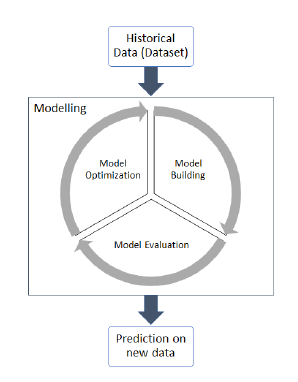
\includegraphics{MLProcess.png}
  \caption{Model Building process} 
  \end{figure}

I modelli di ML assimilano i dati di addestramento,dunque è possibile produrre modelli più precisi basati su tali dati.\\
Un modello di ML è l’output generato quando si addestra il proprio algoritmo con i dati(Figura 1.1); questo modello una volta addestrato sarà in grado di generare un output in base ai dati di addestramento che hanno contribuito alla generazione di esso.\\
Dato l’alto tasso di accuratezza degli approcci di ML e la rapidità in cui il modello può essere generato, ML è usato ogni giorno da milioni di aziende per fare predizioni sulla più efficiente strategia di business.\\
Il processo di ML spesso dipende dalla natura dei dati di training; durante il processo di allenamento, il framework ML è allenato per raggiungere un determinato obiettivo come prendere decisioni, predire un valore o stilare una classificazione.\\
La fase di training permette di scoprire potenziali relazioni tra i dati di input e output senza alcun intervento umano.\\
Esistono anche algoritmi di ML ``online'' nei quali ogni predizione aggiorna il modello per ogni nuova funzione di input.\\
In questo testo studieremo e confronteremo due casi di studi riguardanti la costruzione di questi modelli per problemi diversi, con l’obiettivo di cercare le fasi che accomunano i differenti casi di studio ed analizzarli. 
\end{document}